\chapter{Unifying Logic} \label{uni}
In this chapter we discuss the idea of a unifying logic for the Semantic Web. The term itself stems form the so-called Semantic Web Stack (or Semantic Web Layer Cake).
This schema represents the envisioned architecture for the Semantic Web and the unifying logic is one of its pieces.
Therefore we start with a discussion of that stack in general to then focus on the parts relevant for this thesis. This considerations then lead to the research questions.


\section{The architecture of the Semantic Web}
 To concretely realise the dream of a machine understandable Web as it was envisioned by Tim Berners-Lee et al. \cite{SemanticWeb}, 
an architecture has been proposed, the  
 ``Semantic Web Stack'' (aka ``Semantic Web Layer Cake'').
This stack provides a structural overview of the different concepts, technologies and standards needed for the Semantic Web to become reality. 
Its shape has changed over the years \cite{Gerber2} due to the progress made---several languages such as \rdf \cite{rdf} and SPARQL \cite{sparql} have been standardised---but also 
as a consequence of controversial discussion \cite{twotowers,rearch}. 
Knowing that this version can---and most probably will---evolve and change in the coming years, 
we focus %current 
%version from wikipedia, which is a slight modification of 
on the latest official 
variant %\footnote{Available at: \url{https://www.w3.org/2007/03/layerCake.svg}.} 
 and discuss its different parts. This variant is displayed in Figure~\ref{fig:stack}.\footnote{Colours and shapes are changed in this version to make it fit better into this book. 
The original picture is available at: 
\url{https://www.w3.org/2007/03/layerCake.svg}.
A newer (unofficial) version is for example provided by Hogan \cite{hogan}.} 
\begin{figure}[h!]
	\centering
	%\begin{adjustwidth}{-\marginnotewidth}{}%
	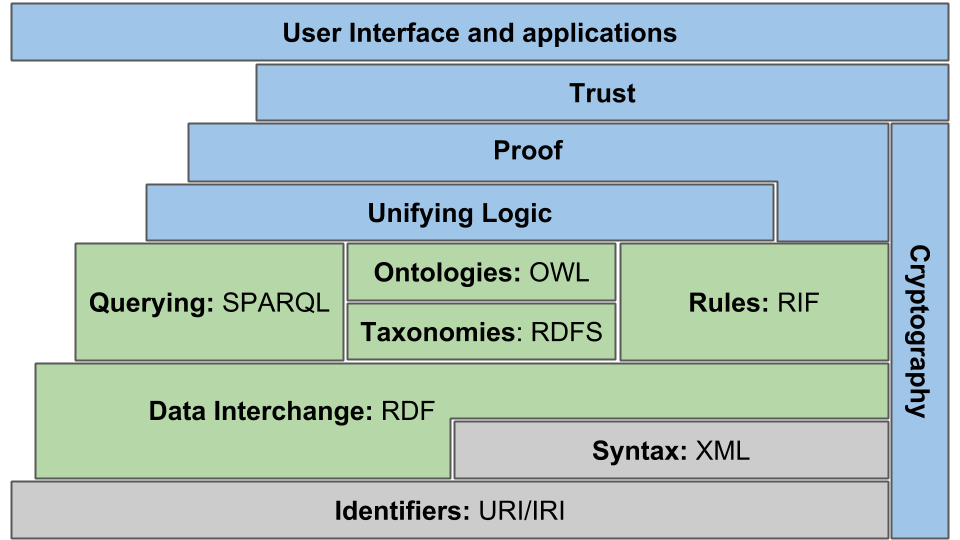
\includegraphics[width=0.8\textwidth]{stack6}
	%\end{adjustwidth}
	\caption[Semantic Web Stack]{Semantic Web Stack.}
	\label{fig:stack}
\end{figure}
%\footnotetext{Source: \url{https://en.wikipedia.org/wiki/Semantic_Web_Stack}}
Each layer placed on top of other layers  depends on  these other layers but not on those above them. Neighbouring layers can, but not necessarily have to make use of each other. 
We go from the bottom of the stack to its top to explain all its elements:

\begin{description}
%  \item[Character Set] To be compatible with the current Web and its applications, but also with textual documents in all languages in general,
%  the Semantic Web relies on Unicode.
 \item[Identifiers] The Semantic Web is a global network which relies on interoperability. In such a big setting, it is crucial that the names of individuals and concepts are unique.
 For their representation Uniform Resource Identifiers (\uris) and Internationalized Resource Identifiers (\iri{}s) are used.  
 \item[Syntax] There are several syntax formats frequently used in the Semantic Web. Standards of the World Wide Web are employed---such as XML or JSON---but also formats 
 only created for the Semantic Web such as for example the Terse RDF Triple Language (Turtle). The fact that the Semantic Web stack only mentions XML and omits 
 other notations which are also used
 is often 
 a point of criticism.\footnote{See for example the discussion at: \url{https://lists.w3.org/Archives/Public/semantic-web/2016Feb/0121.html}.} 
 \item[Data Interchange]
In order to exchange data it must be agreed on  a common structure to express knowledge. This 
structure should not be too complex for a machine to parse but still 
powerful enough to make simple statements and connections. 
In the Semantic Web the Resource Description Framework (\rdf) was developed with 
that goal in mind. Knowledge is expressed using simple triples consisting of subject,
predicate and object. By using unique names (\iri{}s and \uris) connections between different triples are made. 
Ideally, one resulting graph then forms the Semantic Web.
 \item[Taxonomies] For the simple classification of objects and properties the Semantic Web uses the standard \rdf Schema (\rdf{}S). \rdf{}S extends the basic representation format 
 \rdf by several predicates with a predefined meaning such as for example \texttt{rdfs:subclassOf} to denote that one class is a subclass of another. 
 %
 \item[Ontologies]
 The taxonomy already gives some basic information about concepts and individuals in the web. To express more complex things in a fixed way, ontologies are used. 
 Ontologies can be understood as a collection of statements about concepts, classes and individuals using a broad variety of logical predicates which have a fixed meaning for the computer.
 Even though, in that sense a collection of rules over \rdf data could be understood as an ontology,  in the Semantic Web context the term refers to a set of statements written in the Web 
 Ontology Language (\owl). This language is based on description logics and a reasoner can use these statements to draw conclusions.
 %
 \item[Rules] Alternatively to \owl, but also in combination with this standard, there is another way of stating knowledge about concepts and data in the Semantic Web: rules. 
 Having their origin in classical logic programming, rules are used to directly state which triples or patterns of triples can be concluded from given information. To combine rule-based reasoning 
 with \owl reasoning the Semantic Web Rule Language (swrl) can be used. As a general format to exchange different kinds of rules, the Rule Interchange Format (RIF) was created. 
 There are also many other 
 rule-based logics used in the Semantic Web which are not standardised (yet), one of them is \notationthree Logic (\nthreelogic) 
 which is the subject of this thesis.
 %
 \item[Querying] Independently of whether reasoning is performed on \rdf data or not, there are many situations in which a user or an application wants to retrieve information 
 by searching for triples of a certain kind. Therefore, querying is an important part of the Semantic Web. To query data from \rdf the SPARQL Protocol And RDF Query Language (SPARQL) is used.
 \end{description}
 The different layers described so far have---at least up to some point---already been realised---for all building blocks there exist standards. 
 The higher layers we discuss now
are either not realised yet or the community has not yet agreed on a solution (or even on a concrete definition of the problem). 
% In that sense the  following description might be subjective. For alternative views we recommend for example 
% the introduction done by Hogan \cite{hogan}.
 \begin{description}
 \item[Unifying Logic]
 Above these concepts of querying, ontologies and rule based reasoning, there is the layer of a unifying logic: 
 a logical framework which connects the other concepts and makes it possible interoperate between them. 
The logic should thus support the inference mechanisms of these three underlying concepts and the formats below, in particular \rdf.
 \item[Proof]
 Once this unifying logic is found, it should be possible to provide formal proofs for the derivations done using this logic (and thereby also for all derivations of the underlying standards). 
 These proofs should be exchangeable by different parties and it should be possible to automatically check their correctness. Additional information like for example the source of knowledge 
 used could also form part
 of these proofs.
 \item[Cryptography]
 The cryptography layer lies aside of the layers discussed so far. For all the resources and at all layers of the Semantic Web cryptographic techniques should be used 
 to for example verify the identity of an agent or to implement access control mechanisms. Here, existing Web technologies and protocols like for example RSA or HTTPS but 
 also newer techniques like blockchain could be used.
 \item[Trust]
 The layers proof and cryptography together form the base for the trust layer: only if reasoning steps, sources of information and the trustworthiness of all parties involved
 can be verified and manipulation 
 can be excluded, people and machines can trust the information they get from the Semantic Web.
 \item[User interface and applications]
 This highest layer of the stack is also the broadest: a Semantic Web only makes sense if it is more than a scientific construct. 
 It needs to be used by humans but also by different machines which, following
 the original vision, should be able to interact between each other and make use of the resources available. Of course there are already applications making use of the Semantic Web implemented, but
 together with the progress of the Semantic Web as a whole, we expect a lot more to come.
\end{description}

%After having briefly introduced the Semantic Web Stack, it is worth to mention that there are different points which are 
% Introduction given by Hogan \cite{hogan}.
% Gerber \cite{Gerber} \cite{Gerber2}. Really nice: abstracts from technnologies. Bad: the word ``unifying Logic'' dissapeared.
% 
% Ian Horrocks: two towers \cite{twotowers} -- by supporting the closed world assumption we get two semantic webs.
% 
% 
% \cite{rearch} Paper by Boley, Kifer, etc. ``realistic'' architecture, not just one technology. 
% 
% 
% \subsection{Data Interchange}
% RDF
% 
% \cite{rdf}
% \subsection{Querying}
% \subsection{Ontologies}
% RDFS
% OWL
Introducing the Semantic Web stack, its critical points should also be discussed:
One problem which was already mentioned above is that the current stack explicitly names XML as a base for the syntax while many applications rather use formats like 
the JSON based JSON-LD~\cite{jsonld} or the Turtle~\cite{turtle}, which is also easy to read for humans, to represent \rdf.\footnote{Even though in the case of Turtle this point 
is somehow addressed as the \rdf layer directly 
touches the layer of identifiers which are directly used by Turtle.} This point is certainly true, 
but we see the formats occurring in the stack as open lists of formalisms which have already been standardized to serve the purpose mentioned 
rather than a simple declaration of the decision in favour of a format. To emphasize this, we added to every layer which is labelled with a standard also the general purpose this layer 
fulfils. These names are not always present in the original stack our figure is based on.

Other possible problems with the stack can be found in the middle layer: While \owl and SPARQL are concrete logics disposing over their own semantics (see \cite{owlrdfsem,owldsem} 
and \cite{sparql}, respectively), RIF~\cite{rif} is a format to interchange rules and not a logic on its own.
\todo{maybe add online reference for rif? Get the owl citations right}

Here: Problems with Ontology layer

Even the parts realised have certain ``cracks'' or problems. It was mentioned earlier that all higher layers should rely
on the layers beneath them. That said, one would expect that \owl would be compatible with \rdf{}S---and there exists a version which actually is, \owl full. 

Must it even be \emph{one} unifying logic?

\section{The Unifying Logic}



Mention: RDF is only compatible with owl full

\cite{twotowers} think that the rules and owl should not be side by side, they see the open world assumption as problem and want to have the rule layer on top of owl dl.

Maybe also mention that the connection of owl and rdfs is rather artificial -> two semantic definitions...

%\subsection{Rule Based Logics}

History about big discussion open vs. closed world assumption.

Discussion: closed world assumption a problem

comes also in \cite{rearch}.

Solution:scoped negation as failure.

The paper above sees rules without negation as failure such as swrl just as extension of owl and not as belonging to the other format.

rules and owl see each other as black boxes.
we can combine them
-> this reminds me a little bit of validation where we first do dl reasoning and then querying

the paper also see querying as some kind of rule application (I think they are right here).


RIF

SWRL

N3

\cite{N3Logic}

Explain this unifying logic, list the attempts to find one and answer the question: why N3 and not those?



Here or somewhere else mention description logic programs \cite{DLP} which try to combine Description Logic and Logic Programming. - OK, rather their intersection.

\cite{knorr} rules as unifying logic

\cite{unilogic} first attempt to close the rift between rule-based and description logic reasoning, problem remains: open world assumption


What do we expect from the ``unifying logic''?

The vision of the Semantic Web is to enable machines to use the Web just as humans do. For that they need to be able to \emph{understand} and \emph{exchange} data through the Web. 
An unambiguous way to express knowledge is needed, a logic. 
This logic needs to be well defined to avoid misunderstandings and it needs to be agreed on this definition between all possible parties involved.


Different approaches in the ``quest for a unifying logic'': extend owl (nominal schemas, same paper \cite{unilogic}), ``merge'' owl and rules (both mentioned in \cite{unilogic}). We go a third way: rules for all.

approaches consider worst case time complexity (e.g. \cite{unilogic}). -> argue that this is nice but we focus on practical cases.

OWL and rdf is already artificial, rules are natural extension of RDF and the can cover owl.

Later on mention integrity constraints on data bases which are needed for validation.

Artikel von Motnik \cite{DLASP} sagt was ueber default rules for validation -> validation ist ein ziemlich interessantes Thema hier.

unifying logic on application level, not just a construct -> we therefore exclude owl full.

allgemein: answer set programming hat zwei Formen der Nagation.

noch was von Lifschitz und asp zitieren.


Also say why you should go for N3: unifying logic is not just a theoretical construct, it also gives practical advantages: reasoning is often faster when you use only one logic.  

somewhere: reification is not the same as citation.

Knorr hat DL style syntax
It has advantages if you need 
the features of different frameworks. Of course, if you know that, eg only querying is needed you should still go for SPARQL.


% The Unifying Logic needs to be well-defined in itself, it needs to be able to ``understand'' the underlying formats, in particular to query, do DL reasoning and use rules. 
% Additionally it should provide the opportunity to connect to the proof layer.
Requirements:
\begin{description}
 \item[clear semantic definition] 
The meaning of every statement needs to be clearly defined.
 \item[compatibility with existing Web standards]  Existing standards of the Semantic Web need to be supported. 
 In particular, querying, Description Logics, and rule based reasoning need to be covered.
 \item[support of proofs] It must be possible to express, interchange and check all derivations made in the logic.
 \item[capability to handle change] It must be possible to express and reason about change.
\end{description}



\section{Research questions}
Question: Is N3 a suitable candidate to become the unifying logic for the semantic web?

Sub-questions:

Can we give a clear semantic definition of Notation3 Logic?

How does Notation3 Logic interfere with other formats? Can SPARQL, OWL and RIF be expressed?

Is it possible to express proofs in N3?

Can N3 handle change?

I think I need to be more specific. To find that: what do I actually do here?



% \textbf{Part 4: going beyond the limits}
% 
% introduce weighted transition logic to express change
% 
% This part is optional



Somewhere I need to talk about problems, especially decidability and for example the problems of OWL full.

Should I have a chapter about negation as failure?

Problem: blank nodes in SPARQL